%本节的主要内容是讲述一些思考的点和考虑
\section{Considerations}
%在故事线可视化中加入文本中的事件,以及参与事件的各个实体之间的关系,可以更直观的展示蕴涵的信息、更好的解释实体之间的关系和各个实体的功能。为此,我们提出了E^2Storyline,其目标是生成清晰、可读性高,并能展示更多信息的故事线可视化。在本节中,我们将就数据及可视化设计时考虑的因素进行说明。
\noindent Incorporating events into storyline visualization, and the relationships between the various entities involved in the events, allows for a more intuitive presentation of the information contained in the story, better explanation of the relationships between entities and the roles of each entity. For this purpose, we propose $E^2$Storyline, whose goal is to generate storyline visualizations that are legible, intelligible, and demonstrate more information. In this section, the considerations for input data and visualization design are illustrated.

%	3.1   数据要求
\subsection{Data Acquisition Requirements}
%故事发展是有时间脉络的。尽管在小说、电影等艺术性较强的文学作品中时间会有交错的情况,但在社交媒体、网络文字直播等新兴媒体中,时间通常是线性的。一个具有良好线性时间的文本内容可以更好的用故事线可视化进行展示。
\noindent Story development is temporal in nature. While time can be staggered in more artistic literary works such as novels and movies, time is usually linear in emerging media such as social media and live online text. A textual content with good linear time can be better presented with storyline visualization.  

%故事中对某一时刻两个实体之间关系的描写往往需要用一个短句或者一个长句。这种表达方式不够简练。我们需要寻找新的表达方式。新的方式需要具备以下性质:1.它具有结构化的形式。结构化的形式可以减少文本的存储空间,使数据更易处理。2.它能记录参与的实体。记录的实体可以在后续模式探索时发挥作用。3.它能表达实体之间的关系。保留实体间的关系可以减少信息丢失,更易发现实体的行为模式。
The depiction of the relationship between two entities at a given moment in a story often requires a short sentence or a long sentence. Such expressions are not concise enough. For this, we need to find a fresh way of expression. The new approach needs to have the following properties: \ding{182} it has a structured form. The structured form reduces the storage space for text and makes the data easier to handle. \ding{183} it can record the entities involved. The recorded entities can be useful in subsequent model exploration. \ding{184} it can express the relationships between entities. Preserving the relationships between entities reduces information loss and makes it easier to discover the behavior patterns of entities.

%在自然语言处理中,结构为<Subject-Predicate-Object>(SPO)的三元组可以用来编码带有语义数据的句子。SPO三元组中包含了行为属性的施者和受者。尽管是离散抽取SPO三元组的,但其仍具有时间信息,且对整体趋势不会产生干扰。鉴于此,我们可以按照故事中出现的先后顺序,对角色和行为进行SPO三元组抽取。
In natural language processing, a triple with the structure \textit{$<$Subject-Predicate-Object$>$} \textbf{(SPO)}~\cite{hoffart_yago2_2013} can be used to encode sentences with semantic data. An SPO triple contains both the giver(\textit{subject}) and the receiver(\textit{object}) of the action(\textit{predicate}). In view of this, we extracte SPO triples for characters and actions in the order of their appearance in the story. While the SPO triples are extracted discretely, they still have temporal information and the overall trend is not disturbed. In view of this, we extract SPO triads for characters and behaviors in the order of their appearance in the story.

%我们使用了两个真实数据集。一个是欧冠2015-2016赛季16强,巴塞罗那对阵阿森纳第一回合的文字直播数据。该数据具有很强的线性时间性。我们结合赛后集锦寻找比赛中的事件。另一个是电影《纳尼亚传奇》,我们根据现有工作以及电影本身标注事件抽取三元组。
We used two real datasets. One is the live text data from the Champions League 2015-2016 Round of 16, Barcelona vs. Arsenal first leg. The data is highly linear in time. We combine the post-match highlights to find events in the match. The other is the movie \textit{The Chronicles of Narnia}, where we label events to extract SPO triples based on existing work as well as the movie itself.
%	3.2   设计需求
\subsection{Design Requirements}
% 设计需求在各类可视化展现中是普遍存在的,也是至关重要的。针对故事线可视化,根据需求的通用性程度,我们提出了三种不同层级的设计需求。
\noindent Design requirements are ubiquitous and crucial in various visual presentations~\cite{tanahashi_design_2012}. For storyline visualization, we formulated three different levels of design requirements depending on the degree of generality of the requirements.

%	3.2.1	硬需求
\subsubsection{Hard Design Requirements}
%经过多年的发展探索,故事线可视化有多个通用的设计要求。我们将他们定义为硬性设计要求。硬性设计要求是经过众多学者验证并认可的。它们是故事线可视化默认遵守的设计要求。
\noindent After years of development and exploration, storyline visualization has several general Hard Design requirements(\textbf{HDR}). The hard design requirements have been verified and recognized by many scholars. They are design requirements that Storyline Visualization adheres to by default.

%HDR1:用一条随时间发展从左至右延展的线表示实体。线的起始和结尾,表示实体出现和消失的时间点。线的长度表示实体在故事中的寿命。
\ding{118}  \textbf{HDR1: An entity is represented by a line extending from left to right over time.} The start and end of the line, indicating the points in time when the entity appears and disappears. The length of the line represents the lifespan of the entity in the story.

%HDR2:用线条的聚集和发散表示实体是否参与同一个事件。如果某段时间某些实体参与了同一个事件,代表这些实体的线就会聚在一起。反之则会发散,或者不会有明显的聚集过程。
\ding{118}  \textbf{HDR2: Use the aggregation and divergence of lines to indicate whether entities participate in the same event.} If certain entities participate in the same event at a certain time, the lines representing those entities will come together. Otherwise, it will diverge, or there will be no obvious aggregation process.

%如图HDR.a:解释HDR1,蓝色的线表示Entity ※, 橙色箭头表示时间。图HDR.b:解释了HDR2,实体A、B、C和D分别用绿色、紫色、橙色和红色表示。在T1时刻,实体B和C有关系,因此它们聚集在一起;在T2时刻,实体A和B有关系,实体C和D有关系,而实体B和C没有关系,因此实体B和C分开,分别与实体A和D聚集。
Fig~\ref{fig:HDR}.a illustrates \textbf{HDR1}. The blue line and the orange arrow represent Entity$\divideontimes$ and time, respectively; Fig~\ref{fig:HDR}.b illustrates \textbf{HDR2}. Entities A, B, C, and D are represented in green, purple, orange, and red, respectively. At time T1, entities B and C have a relationship, so they are clustered together; at time T2, entities A and B have a relationship, entities C and D have a relationship, but entities B and C have no relationship. So entities B and C are separated and aggregated with entities A and D, respectively.

%HDR的示意图。
\begin{figure}[h]
	\centering	
	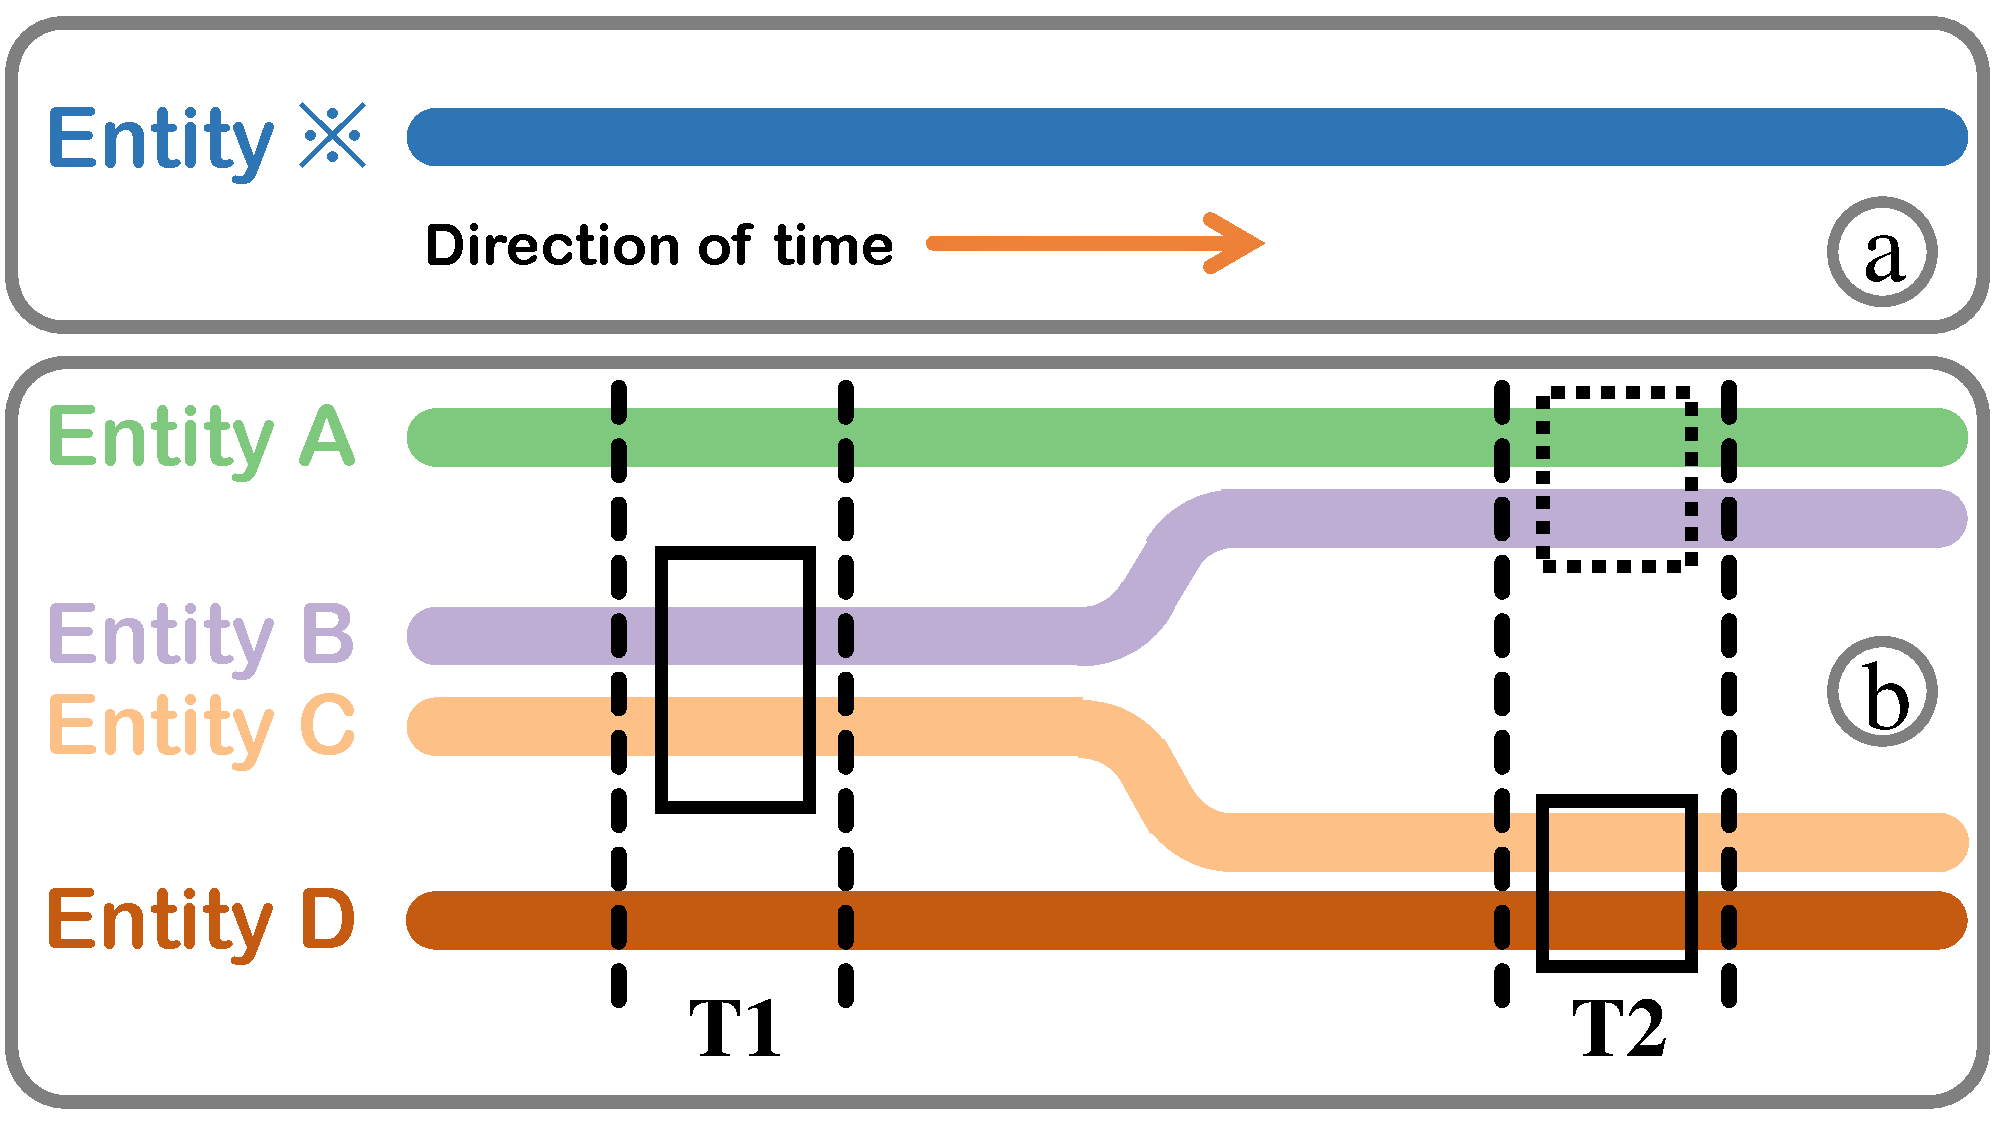
\includegraphics[width=0.38\textwidth]{Fig/HDR.pdf}
	\vspace{-0.5em}
	\caption{Schematic of HDR.}
	\vspace{-1.5em}
	\label{fig:HDR}
\end{figure}

%	3.2.2	软需求
\subsubsection{Soft Design Requirements}
%故事线可视化作为一种向用户传递信息的表达方式,简洁直观是十分重要。为了达到这个目标,研究人员在遵守硬性设计要求的基础上,还要遵守不同的软性设计要求。软性设计要求是指,设计要求相同,但实现的方式可以不同。比较常见的软性设计要求有以下几个:
\noindent As a way of conveying information to users, storyline visualization is very important to be concise and intuitive. In order to achieve this goal, researchers must comply with different Soft Design Requirements(\textbf{SDR}) in addition to hard design requirements. Soft design requirements mean that the design requirements are the same, but the implementation can be different. The more common soft design requirements are as follows:  

%SDR1:减少线交叉个数。较少的线交叉可以降低视图的复杂程度,减少用户阅读负担,更好的理解视图中蕴含的信息。
\ding{117}  \textbf{SDR1: Reduce the number of line crossings.} Fewer line crossings can reduce the complexity of the view, reduce the user's reading burden, and better understand the information contained in the view.

%SDR2:减少线摆动次数。过多的或者没必要的线摆动,不仅在视觉上会产生线条的不连续性,同时还会变相增加线交叉个数。
\ding{117}  \textbf{SDR2: Reduce the number of line swings.} Excessive or unnecessary line swings will not only visually produce line discontinuities, but also increase the number of line crossings in disguised form.

%	3.2.3	自定义需求
\subsubsection{Custom Design Requirements}
%为了在故事线可视化中展现实体与实体之间的关系,即格式为(实体-关系-实体)的三元组,本文除了遵守上述设计要求外,还增加了一些自定义设计要求。
\noindent In order to show the relationship between entities and entities in the visualization of the storyline, that is, the triples in the format $<$entity-relation-entity$>$, in addition to complying with the above design requirements, we also adds some Custom Design Requirements(\textbf{CDR}).

%CDR1:使用矩形像素图用来表现事件。像素图中,每一行是同个实体,每一列代表一个三元组,从左至右是时间方向。
\ding{108}  \textbf{CDR1: Use rectangular pixmaps to represent events.} In the pixmap, each row is the same entity, each column represents a triple, and the time direction is from left to right.

%CDR2:同一事件中同一个SPO三元组的实体之间尽可能靠近。让事件显得紧凑,可以使用户更为便捷地发现有关系的实体。 
\ding{108}  \textbf{CDR2: Entities of the same SPO triplet in the same event are as close as possible to each other.} Keeping events compact makes it easier for users to discover related entities.

%针对我们提出的自定义设计要求,在图CDR中进行了详细地说明。在图CDR.a中,x轴的正向是时间方向,y轴是实体排列的位置。灰色框内的像素图代表事件。像素图的每一列代表一个三元组。例如,图中第一列实体A和实体C之间有关系,我们将对应的位置填上与对应实体相同的颜色,剩余的位置留白,以此类推。图CDR.b所示是满足我们提出的两个CDR的结果之一。我们可以发现,像素图的杂乱程度有显著减少,增强了事件的可读性,同时用户可以更好的理解单个事件中实体之间的关系以及某个具体实体的作用。
The \textbf{CDR} we put forward are illustrated in detail in Fig~\ref{fig:CDR}. In Fig~\ref{fig:CDR}.a, the positive direction of the x-axis is the time direction, and the y-axis is where the entities are arranged. The pixmap inside the grey box represents the event. Each column of the pixmap represents a triple. For example, there is a relationship between entity A and entity C in the first column of the figure. We fill in the corresponding position with the same color as the corresponding entity, and leave the remaining positions blank, and so on. Fig~\ref{fig:CDR}.b shows one of the results satisfying our two proposed \textbf{CDR}s. We can find that the clutter of the pixmap is significantly reduced, the readability of events is enhanced, and users can better understand the relationship between entities in a single event and the role of a specific entity.

%CDR的示意图。
\begin{figure}[h]
	\centering	
	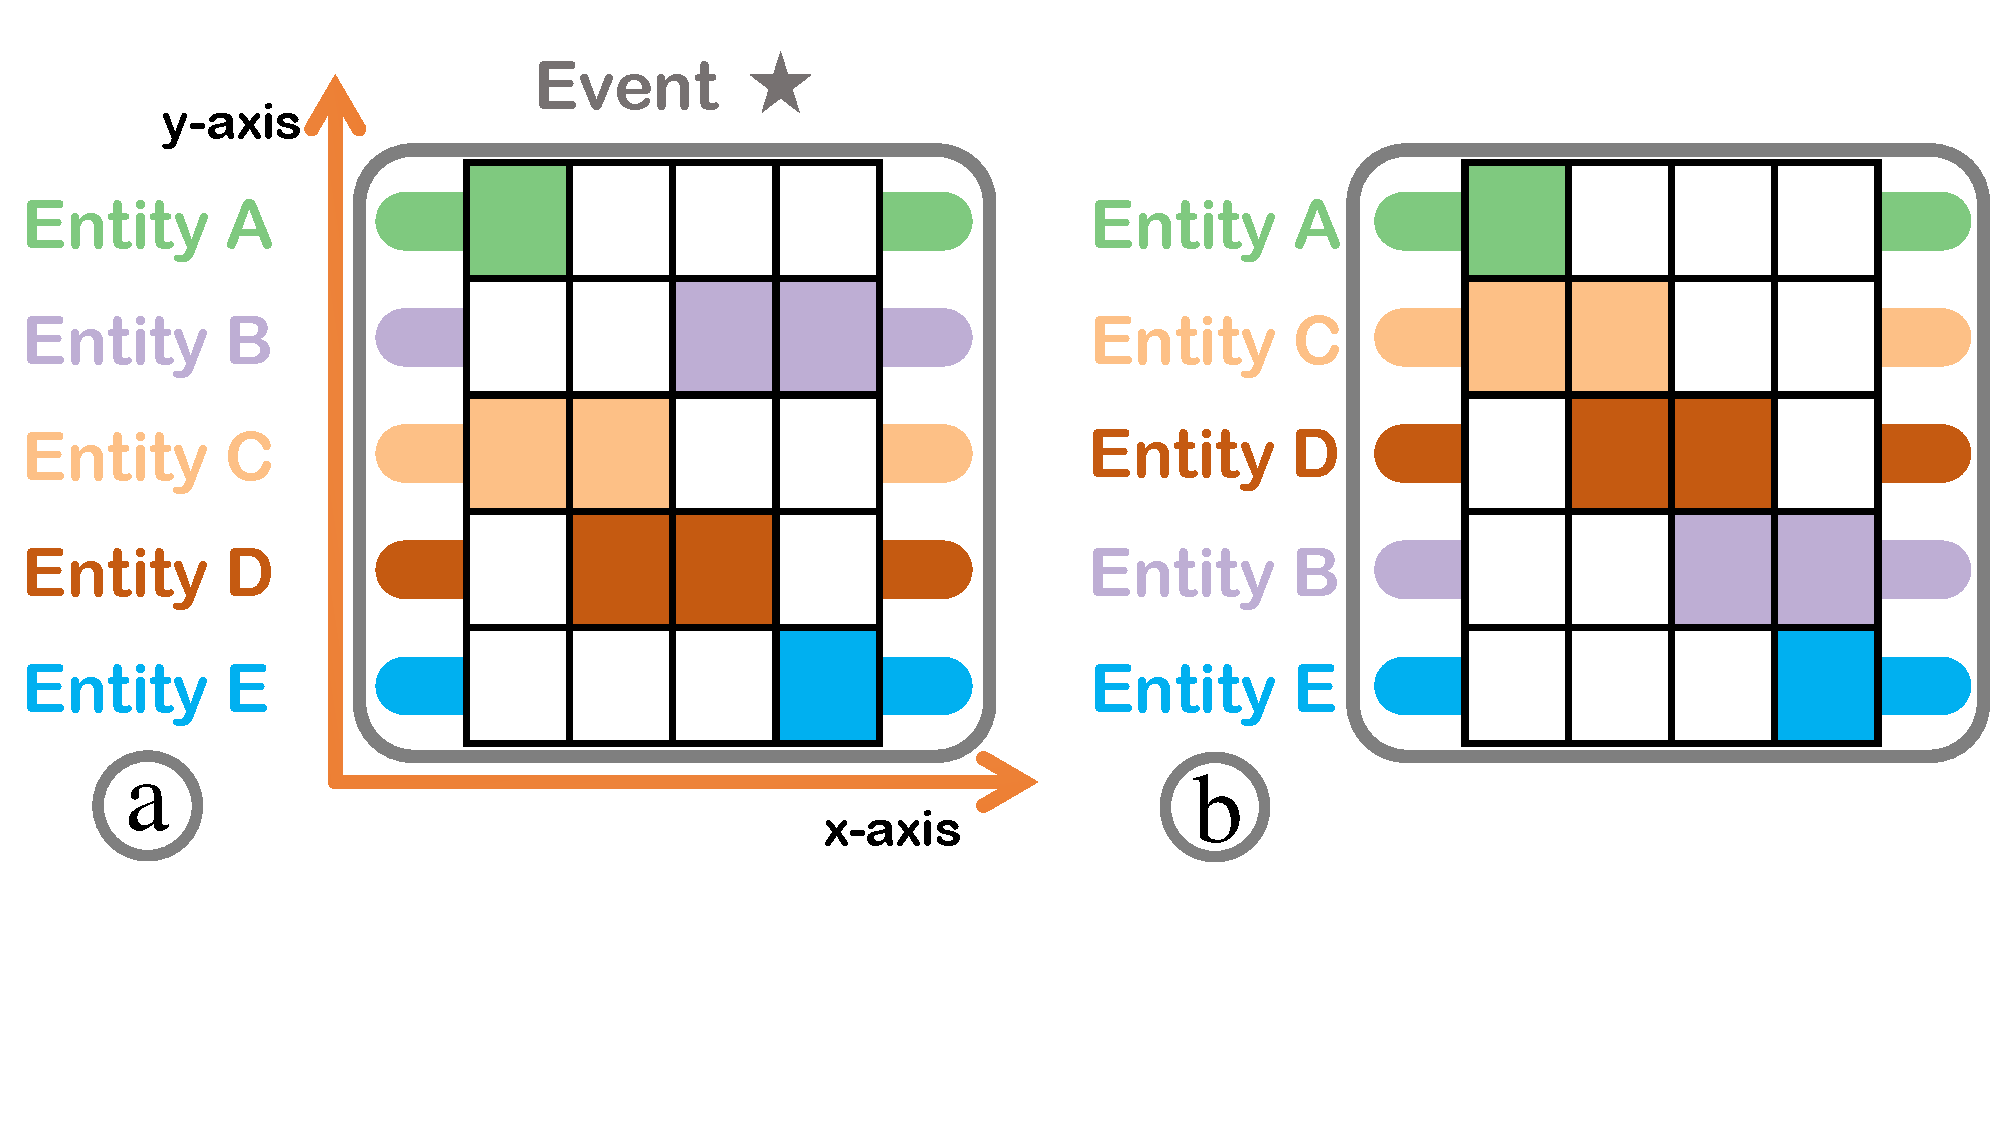
\includegraphics[width=0.48\textwidth]{Fig/CDR.pdf}
	\vspace{-3.0em}
	\caption{Schematic of CDR.}
	\vspace{-1.5em}
	\label{fig:CDR}
\end{figure}